\chapter{Aplikacja}
Projekt zaczęto realizować w~lipcu 2020. Prace koncepcyjne oraz pozyskiwanie wiedzy zrealizowano w~sierpniu 2020, a~wynikiem tych działań było uruchomienie tablicy Trello. Trello to internetowy serwis, którego główną funkcją są tablice organizacji projektów. Tablica zawierała zadania deweloperskie, ale także organizacyjne. Cały projekt był prowadzony w~metodyce Scrum. Metodyka została dostosowana do charakteru oraz wielkości projektu. W~pierwszej połowie projektu regularne spotkania odbywały się co dwa tygodnie. W~drugiej połowie, gdzie przeważały szczegółowe zadania techniczne, spotkania odbywały się co tydzień. W~celu przechowywania kodu oraz kontroli wersji użyto technologii Git i~GitHub.
\section{System oznaczania zębów}
\subsection{Wymagania}
Podczas planowania projektu założono minimalne wymagania produktowe - MVP. Wymagania minimalne były kluczowym dokumentem przy regularnym planowaniu prac. Dla systemu oznaczania zębów postawiono takie założenia:
\begin{itemize}
    \item Diagram zębowy z~możliwością wprowadzania danych za pomocą myszki
    \item Przechowywanie informacji w~bazie danych
    \item Eksportowanie danych
\end{itemize} 
Stworzono diagram zębowy w~nowoczesnym stylu graficznym. Wprowadzanie danych jest możliwe za pomocą myszki ale także za pomocą interfejsu głosowego. Komendy głosowe pozwalają lekarzowi uzupełniać diagram zębowy podczas wizyty pacjenta. Taka funkcjonalność nie pojawia się w~innych tego typu produktach na rynku polskim. Dane są przechowywane w~nierelacyjnej bazie danych. Użyto technologii MongoDB. Zaletą nierelacyjnej bazy jest łatwość w~zmienianiu modeli i~struktur danych. Eksport danych jest możliwy na dwa sposoby. Pierwszy dotyczy udostępniania danych, zawartych na diagramie zębowym, pacjentowi. Sposób polega na możliwości wydrukowania diagramu do pliku PDF albo, wprost poprzez drukarkę sieciową, do formy papierowej. Podsumowując, spełniono minimalne wymagania produktowe. Jest to wskazanie na poprawne poprowadzenie projektu. 

Innymi wymaganiami, które opisano we wczesnym etapie projektu, były wymagania pozafunkcjonalne. Określono takie wymagania jak:
\begin{itemize}
    \item Użyteczność - możliwość przyswojenia działania systemu w~ciągu jednej godziny
    \item Kompatybilność - konieczność działania na każdej współczesnej przeglądarce internetowej
    \item Łatwość utrzymania - możliwość rozbudowania aplikacji o~dodatkowe moduły
    \item Bezpieczeństwo - uwierzytelnianie i~autoryzacja przed dostępem do danych
\end{itemize} 
W celu spełnienia założenia użyteczności zwrócono uwagę na prosty projekt graficzny. Cała aplikacja działa w~języku polskim, w~tym interfejs głosowy. Najbardziej skomplikowanym systemem dla użytkownika jest wprowadzanie komend głosowych. Sporządzono film instruktażowy oraz instrukcje użytkowania z~przykładami. Wymaganie kompatybilności zostało rozwiązane przez użycie nowoczesnych technologii opisanych w~rozdziale trzecim. Aplikacja została przetestowana, z~wynikiem pozytywnym, na sześciu nowoczesnych przeglądarkach. Opis testów jest zawarty w~dalszej części pracy. Łatwość utrzymania spełniono poprzez zbudowanie aplikacji na podstawie stylu REST. Aplikacja za pomocą interfejsu i~systemu węzłów końcowych, jest w~stanie rozszerzyć swoją funkcjonalność w~prosty sposób. Wymaganie bezpieczeństwa nie zostało spełnione. Ze względu na niedokładne oszacowanie poziomu skomplikowania implementacji systemów uwierzytelniania i~autoryzacji.

Wymaganie użyteczności, zostało opracowane w~dodatkowy, rozszerzony sposób na podstawie ISO25010. Poczyniono założenia:
\begin{itemize}
    \item Rozpoznawalność zastosowania - ściśle określona funkcja oprogramowania
    \item Łatwość nauczenia się - prostota aplikacji oraz użycie grafik branżowych, dobrze znanych potencjalnym klientom
    \item Ochrona użytkownika przed błędami - prostota aplikacji oraz zastosowanie walidacji pól
    \item Estetyka interfejsu użytkownika - zastosowanie najnowszych technologii, ale ważniejsza jest funkcjonalność
    \item Dostępność personalna - produkt ma sprecyzowaną grupę odbiorców, którzy posiadają podobne umiejętności
\end{itemize} 
Wszystkie z~opisanych powyżej założeń zostały spełnione. Dokładniejsza analiza funkcjonalności została opisana w~pracy wcześniej.


\subsection{Design}

Podczas tworzenia projektu graficznego modułu diagramu zębowego skupiono się na estetyce interfejsu użytkownika oraz jego nowoczesnym designie. Położono także nacisk na możliwie prostą formę ekranów, by ich obsługa nie była dla użytkownika barierą, ale by okazała się jak najbardziej intuicyjna. Szczególną uwagę skupiono na wyglądzie pojedynczego zęba oraz całego diagramu.

Moduł diagramu zębowego składa się z~dwóch głównych części. Pierwszą z~nich jest ekran prezentujący dane osobowe oraz kontaktowe pacjenta. Układ formularza jest przejrzysty i~dzięki takiemu rozwiązaniu - prezentacji danych w~edytowalnych polach - użytkownik jest w~stanie w~prosty sposób przeglądać i~jednocześnie aktualizować wcześniej wprowadzone dane w~jednym miejscu. Obowiązkowe do uzupełnienia dane w~formularzu są walidowane. Sprawdzana jest poprawność nanoszonych zmian, by dodatkowo ułatwić pracę użytkownikom i~pomóc im uniknąć błędów oraz związanych z~nimi ewentualnych konsekwencji.

Drugi ekran pozwala na prezentację oraz edycję danych dotyczących stanu uzębienia pacjenta. Projekt graficzny diagramu zębowego wykorzystanego w~aplikacji powstał na podstawie istniejących diagramów papierowych (Rysunek \ref{fig:karta}) oraz cyfrowych (Rysunek \ref{fig:diagramy}) używanych w~gabinetach stomatologicznych, a~także na podstawie konsultacji z~czynnym zawodowo stomatologiem. Ważne było, by był on jak najbardziej zbliżony do diagramów już wykorzystywanych w służbie zdrowia, tak by ułatwić pracę i~naukę obsługi nowego oprogramowania stomatologom, ale jednocześnie, by sprawdził się w~aplikacji desktopowej.

\begin{figure}[t!]
\centering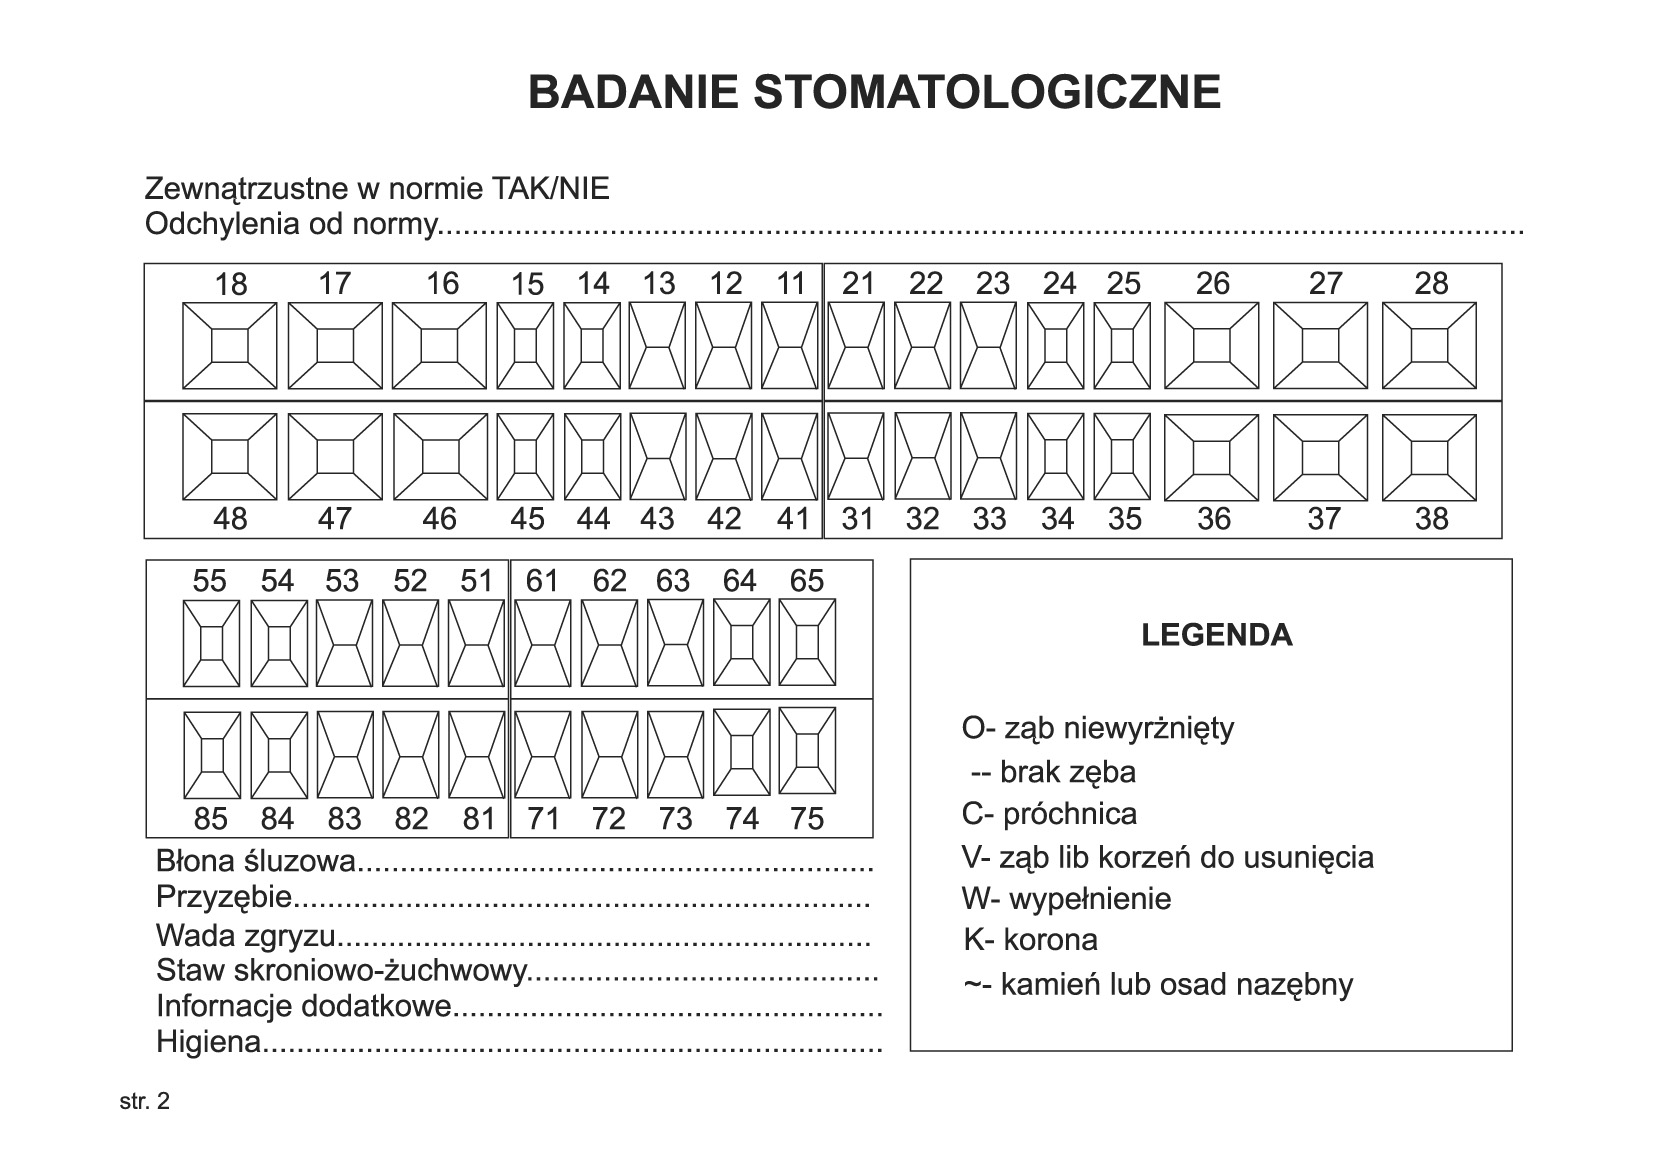
\includegraphics[width=\textwidth]{figures/karta.jpg}
\caption{Przykładowy diagram papierowy wykorzystywany w gabinetach stomatologicznych.\cite{Roydental}}
\label{fig:karta}
\end{figure}

\begin{figure}[t!]
\centering
\subfloat Diagram zębowy w programie eRUM\cite{eRUM}{\label{odnosnik}
\includegraphics[width=\textwidth]{figures/eRum.png}}
\quad
\subfloat Diagram zębowy w systemie Mediporta\cite{Mediporta}{\label{odnosnik}
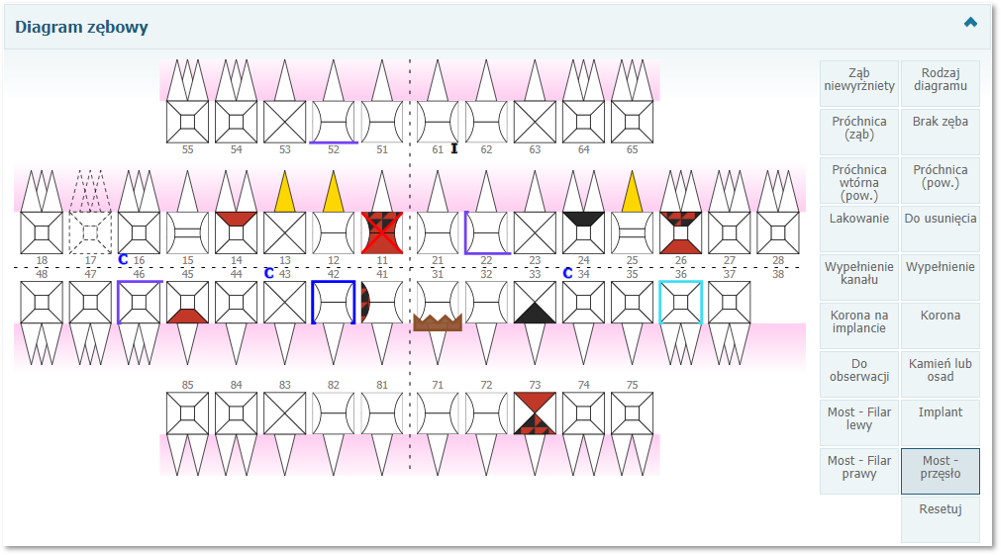
\includegraphics[width=\textwidth]{figures/mediporta.png}}
\caption{Diagramy wybranych aplikacji ułatwiających pracę stomatologom.}
\label{fig:diagramy}
\end{figure}

Diagramy wykorzystywane przez stomatologów bazują zarówno na kwadratowym jak i~okrągłym schemacie opisu zęba. Przy wyborze kształtu opisu wykorzystanego w~aplikacji kierowano się łatwością zaznaczania - możliwością szybkiego wyboru jednego elementu myszką, przejrzystością prezentowanych danych oraz ich estetyką. Ostatecznie w~aplikacji wykorzystano kwadratowy opis poszczególnych zębów. Każdy ząb składa się z~pięciu odrębnych części reprezentujących jego powierzchnie. By zwiększyć czytelność schematu, inaczej przedstawiono siekacze i~kły obu łuków - zwracając uwagę na ich nieduży brzeg sieczny, a~inaczej przedtrzonowce oraz trzonowce, uwydatniając ich powierzchnie zgryzowe.

Podczas tworzenia aplikacji i~projektowania jej interfejsu dużo uwagi poświęcono także detalom. Operacje wykonywane przez użytkownika są często potwierdzane i~opisywane w~widocznym miejscu przez system, by informować na bieżąco o~wprowadzanych zmianach. Takie elementy interfejsu pomagają w~prawidłowym użytkowaniu programu i~w pewien sposób prowadzą użytkownika. Co ważne, osoby korzystające z~aplikacji otrzymują także dodatkowe komunikaty podczas korzystania z~interfejsu głosowego dostępnego w~aplikacji.

Dokładny schemat działania ekranów oraz ich wygląd został omówiony w sekcji \textit{5.1.6 Działanie aplikacji}.



\subsection{Proces instalacji i~uruchomienia}

kurde, nie wiem czy opisywać readme

bo nie wiem czy ta aplikacja nie powinna być prostsza do uruchomienia

niby jest prosta bo się wchodzi przez przeglądarkę ale instalacja bibliotek i~uruchomienie bazy, flaska i~nodejs - jest skomplikowane, ale prostsze już nie będzie 

 - hmm. sama nie wiem. może w~takim razie jedynie wzmianka o~dokładnym opisie w~readme w~repozytorium?






\subsection{Trudności}
Podczas prac deweloperskich napotkano na problemy w~implementacji, niektórych założeń projektowych. W~celu przejrzystości i~wygody pracy, do raportowania problemów użyto GitHub Issues. Jest to system zgłaszania i~opisywania nieprawidłowości w~repozytoriach umieszczony w~serwisie GitHub. Poniżej przedstawiono główne trudności techniczne. 

\begin{itemize}
    \item Wykrywanie urządzeń zewnętrznych - korzystanie z~interfejsu głosowego wymaga użycia mikrofonu. Problemem był wybór odpowiedniego urządzenia przez skrypt pobierający nagrania dźwiękowe. W~systemie występuje wiele urządzeń wewnętrznych i~zewnętrznych. Posiadają one też różne standardy. Przykładowy, niepełny spis widać na rysunku nr 5.1.
    \begin{figure}[ht!]
    \centering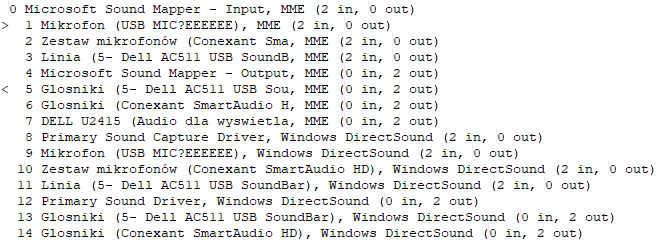
\includegraphics[width=145mm,scale=1.5]{figures/devices.PNG}
    \caption{Spis urządzeń dźwiękowych na maszynie serwera.}
    \label{fig:devices}
    \end{figure}
    
    Rozwiązaniem było automatyczne ustawianie urządzeń na takie jakie w~danym momencie używa system operacyjny.
    \item Nazewnictwo chorób i~powierzchni zęba - w~terminologii stomatologicznej, niektóre obiekty mogą mieć klika nazw. To samo dotyczy się powierzchni zęba. Sprawiało to problemy przy przetwarzaniu komend głosowych. W~celu rozwiązania problemu, stworzono słowniki w~bazie danych. Słownik zawiera zbiór terminów i~ich tłumaczeń. Jeżeli dany obiekt miał kilka nazw, jedna z~nich została wybrana na główną. Reszta nazw jest tłumaczona na nazwę główną. Pozwala to na ujednolicenie interfejsu komunikacji miedzy serwerem, bazą danych i~klientem.
    \item Asynchroniczne przetwarzanie danych - aplikacja klienta wymaga sprawnego przekazywania danych między komponentami aplikacji. Wyzwaniem jest jednak natychmiastowe reagowanie interfejsu graficznego na komendy głosowe lub zmianę wersji danych. Z uwagi na rożne sposoby użytkowania danych, logika klienta jest zaawansowana. Rozwiązano ten problem korzystając z~pełni możliwości technologii Vue, w~temacie działań asynchronicznych. Opis działania technologii można znaleźć w~rozdziale trzecim. 
\end{itemize}

\subsection{Testy}
Aplikacja była testowana po każdej dużej zmianie w~kodzie źródłowym. Testy manualne były przeprowadzane zgodnie z~opisanymi scenariuszami. Scenariusze były rozbudowywane wraz z~aplikacją. Dodatkowo cały system został przetestowany przez pięć osób spoza zespołu deweloperskiego.

Przykładowym punktem scenariusza testowego, był spis komend głosowych. Spis zbudowano w~taki sposób aby zawierał wszystkie słowa zawarte w~bazie danych. Wśród komend były też komendy niepoprawne, w~celu sprawdzenia obsługi błędów użytkownika. Najwięcej testów oraz poprawek dotyczyło interfejsu głosowego. Poniżej przedstawiono zmiany wprowadzone w~systemie komend głosowych, na podstawie testowania aplikacji.
\begin{itemize}
    \item Odmiana słów - każdy użytkownik wypowiada słowa w~unikalny sposób. W~związku z~tym, Google Speech Recognition może nie prawidłowo rozpoznać słowo. Dodatkową trudnością jest nienaturalny ciąg słów w~komendach głosowych np. ,,dwadzieścia jeden sieczna niewyrżnięty''. Z powodu tej nienaturalności system firmy Google może mieć problemy z~użyciem modelu językowego, opisanego w~rozdziale drugim. Efektem może być zrozumienie wspomnianej komendy jako ,,dwadzieścia jeden sieczna niewyrżnięte''. Dla człowieka różnica jest nieznacząca, ale dla komputera jest to inna komenda. W~celu rozwiązania tego problemu zaimplementowano słowniki, o~których budowie wspomniano wcześniej. Dla przykładu, zawartością słownika dla słowa ,,niewyrżnięty'' jest:  ,,niewyrżnięty'', ,,niewyrżnięte'', ,,niewyrżniętych'' i~,,niewyrośnięty''. Wypisane słowa zostały dodane do słownika na podstawie zwróconych przez system słów podczas testów. Analogicznie powstał słownik dla powierzchni zęba. Przykładowo słowa ,,b'', ,,żująca'', ,,żujące'', ,,żując'', ,,sieczna'', ,,sieczny'', ,,sieczne'', ,,siecznych'', oznaczają powierzchnie zęba o~kodzie ,,B''. Kodowanie powierzchni zostało opisane wcześniej w~rozdziale czwartym.
    \item Błąd mikrofonu - uruchomiony interfejs głosowy będzie pobierał komendy w~pętli. W~pierwszej wersji interfejsu głosowego pętla kończyła się po wypowiedzeniu komendy ,,stop''. Problemem była sytuacja, w~której na maszynie serwera nie działał mikrofon. Oznaczało to, że nie dało się zakończyć pętli pobierania komend. Rozwiązaniem było dodanie przycisku dezaktywacji systemu głosowego.
    \item Czas nagrywania komend - system nagrywania oczekuje na pierwszy dźwięk przez dziesięć sekund, następnie każda fraza może trwać do pięć sekund, a~cisza między frazami maksymalnie półtora sekundy. W~pierwszej wersji aplikacji użytkownik nie był informowany kiedy nagrywanie rozpoczyna się i~kończy. Efektem było wypowiadanie dwóch komend podczas jednej sekwencji nagrywania, co kończyło się niepoprawną komendą. Rozwiązano ten problem dodaniem dźwięku startu i~końca nagrywania. Dodano także dźwięk ,,Powtórz komendę.'', w~przypadku podania przez użytkownika błędnej komendy. 
\end{itemize}

Analogicznie na podstawie testów dodano zmiany do warstwy graficznej i~logicznej klienta.

\begin{itemize}
    \item Wielkość grafiki zęba - na diagramie zębów stałych znajdują się aż 32 zębów. Testy wykazały problemy z~wskazaniem myszką w~odpowiednią powierzchnię zęba. Problem rozwiązano za pomocą powiększania zęba. W~momencie najechania myszką na dany ząb, jest on powiększany. Po wykonaniu powtórnie testów zauważono znaczną poprawę w~użytkowaniu diagramu zębowego. Na rysunku \ref{fig:zabPowiekszenie} widać porównanie wielkości przed i~po powiększeniu zęba.
    \begin{figure}[ht!]
    \centering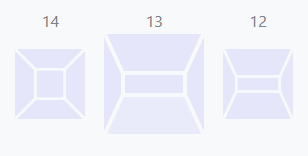
\includegraphics[width=80mm,scale=1.5]{figures/zabPowiekszony.PNG}
    \caption{Porównanie wielkości grafiki zębów przy najechaniu zęba nr 13 wskaźnikiem myszy.}
    \label{fig:zabPowiekszenie}
    \end{figure}
    \item Walidacje pól - na widoku danych osobowych znajduję się wiele pól. Większość z~nich jest opcjonalna. Pola PESEL, imię, nazwisko są obowiązkowe i~podlegają walidacji. Ponieważ jak wykazały testy, użytkownik może zapomnieć uzupełnić numeru PESEL przed zapisem danych. Walidacja numeru PESEL znalazła się także na formatce do wyszukiwania danych pacjentów.
    \item Wersjonowanie - podczas testów zwrócono uwagę na potrzebę przeglądania historii zmian w~diagramach zębowych. Historia zmian rozumiana jest jako historia wizyt pacjenta. W~związku z~tym, dodano proces wersjonowania oraz nowe przyciski na widoku diagramu. Sam proces został dokładnie opisany w~rozdziale czwartym.
\end{itemize}

Poniżej podano przykładowy scenariusz testowy, który użyto do testów.

\begin{enumerate}
    \item W~formatce ,,Podaj pesel'' wprowadź wartość ,,87101912345'', kliknij przycisk ,,Wybierz osobę'' - powinny załadować się dane pacjenta.
    \item Ustaw pole ,,Pesel'' na ,,123'', kliknij ,,Zapisz dane'' - zapis powinien być niemożliwy.
    \item Ustaw pole ,,Pesel'' na ,,87101912345''.
    \item Przejdź na widok diagramu zębów stałych.
    \item Ustaw, klikając myszką, cały ząb o~numerze 14 na ,,Ubytek'' - ząb powinien być cały żółty.
    \item Włącz interfejs głosowy.
    \item Wypowiedz komendę ,,18 bliższa wypełnienie''.
    \item Wypowiedz komendę ,,17 żująca ubytek''.
    \item Wypowiedz komendę ,,46 sieczna próchnica''.
    \item Wypowiedz komendę ,,22 cały most''.
    \item Wypowiedz komendę ,,33 policzkowa ubytek''.
    \item Wypowiedz komendę ,,33 cały usunięty''.
    \item Wypowiedz komendę ,,14 test test'' - system powinien poprosić o~powtórzenie komendy.
    \item Wypowiedz komendę ,,14 cały zdrowy''.
    \item Wypowiedz komendę ,,stop''.
    \item Wróć do widoku danych osobowych i~zapisz dane.
\end{enumerate}
    Podany scenariusz testowy zawiera dodatkowo obraz poprawnego diagramu zębowy. Po przejściu powyższego scenariusza, wygląd diagramu jest zaprezentowany na rysunku \ref{fig:zebyTest}. Dodatkowo programista po każdym przejściu scenariusz sprawdzał poprawność dokumentów na bazie danych, a~także konsole błędów wszystkich komponentów aplikacji.
        \begin{figure}[ht!]
    \centering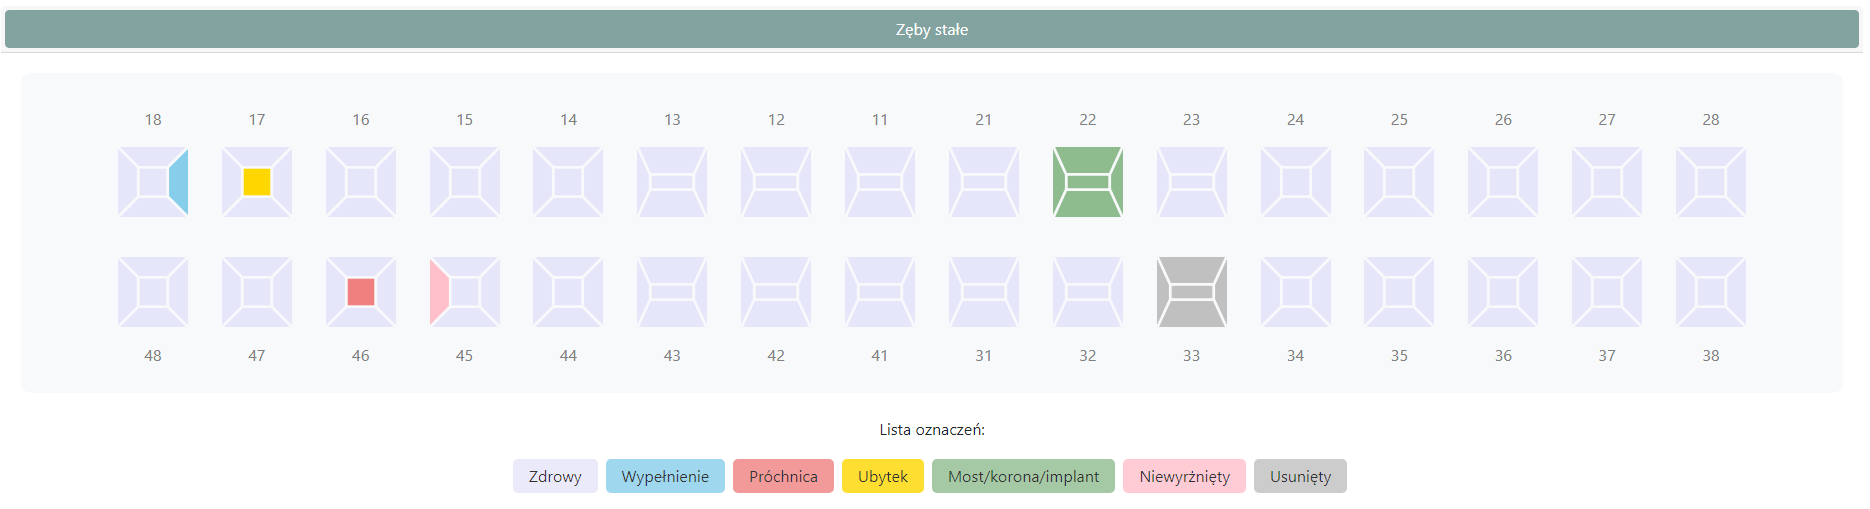
\includegraphics[width=145mm,scale=1.5]{figures/zebyTest.PNG}
    \caption{Poprawny efekt końcowy przykładowego scenariusza testowego.}
    \label{fig:zebyTest}
    \end{figure}

\subsection{Działanie aplikacji}

Aplikacja realizująca moduł diagramu zębowego składa się z dwóch głównych widoków, co zostało opisane w sekcjach wcześniejszych. Pierwszym z nich jest ekran umożliwiający zapis oraz prezentację informacji o pacjencie - jego danych osobowych oraz kontaktowych, drugim - ekran prezentujący diagram zębowy, obrazujący stan uzębienia pacjenta z uwzględnieniem zarówno jego zębów stałych, jak i mlecznych. Poniżej znajduje się dokładny opis wymienionych ekranów.

\subsubsection{Dane osobowe}

Pierwszy widok aplikacji to zakładka \textit{Dane osobowe}. W górnej części umożliwia ona wczytanie wcześniej zapisanych danych. By wyświetlić dane pacjenta, który został już dodany do bazy, należy wprowadzić w wyznaczonym miejscu jego pesel, a następnie zatwierdzić go przyciskiem \textit{Wybierz osobę}. Dane zostaną wówczas wczytane i wyświetlone w formularzu znajdującym się niżej. Forma ta umożliwia jednoczesną prezentację danych z możliwością łatwej ich edycji. Informacjami, które są wymagane, by zapisać dane o pacjencie są pierwsze imię, nazwisko oraz pesel. Sprawdzana jest poprawność tych pól, a efekt walidacji oznaczany jest kolorami zielonym lub czerwonym. Uzupełnienie pozostałych informacji jest opcjonalne i nie uniemożliwia zapisu do bazy danych.

\begin{figure}[ht!]
\centering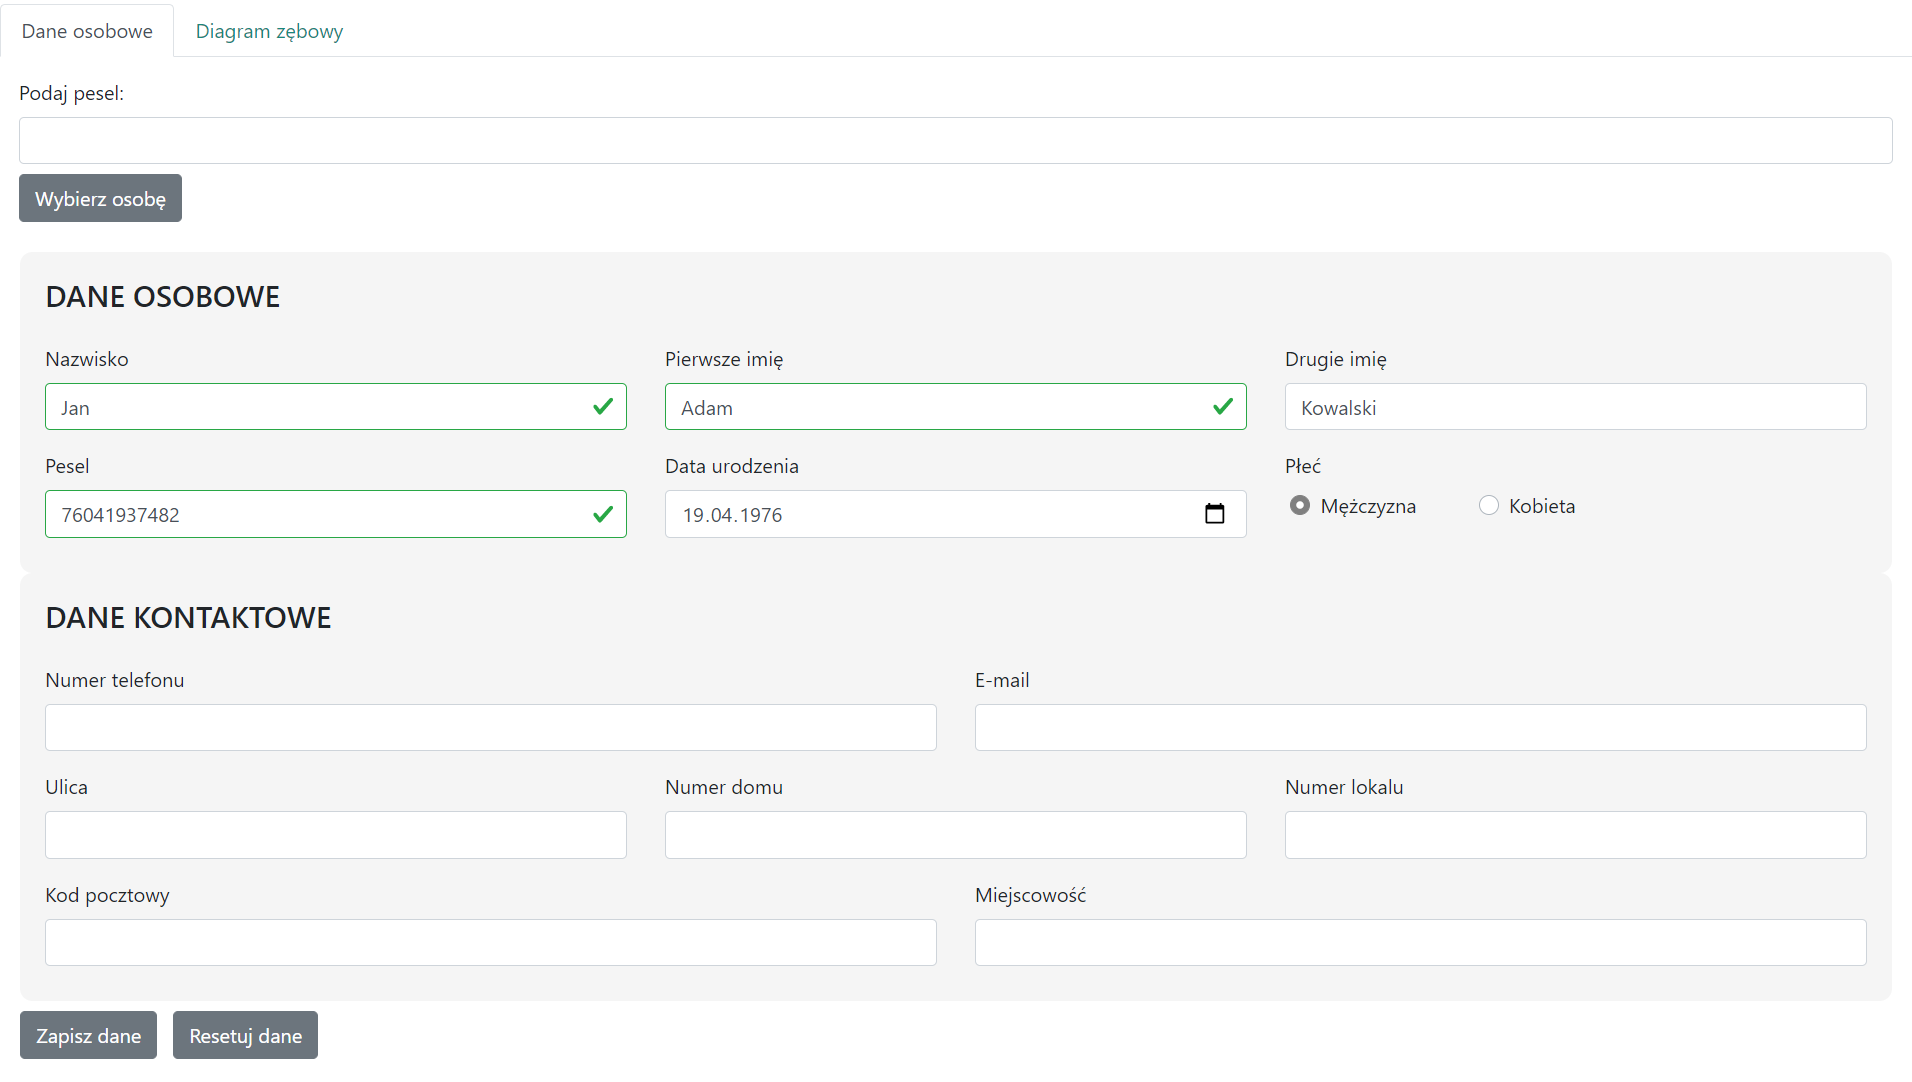
\includegraphics[width=\textwidth]{figures/fromularz.PNG}
\caption{Ekran umożliwiający wprowadzanie do systemu nowych pacjentów oraz przeglądanie i~edycję wcześniej zapisanych danych. \textcolor{red}{błąd!}}
\label{fig:examleForm}
\end{figure}

Widok ten umożliwia także dodanie do bazy nowego pacjenta, którego dane jeszcze się tam nie znajdują. W tym celu należy pominąć pole umożliwiające wprowadzenie szukanego peselu, a jedynie poprawnie uzupełnić prezentowany formularz.

Na dole strony znajdują się dwa przyciski - umożliwiające kolejno zapis lub reset wprowadzonych danych. Po naciśnięciu każdego z nich użytkownik proszony jest o potwierdzenie wybranej operacji. Potwierdzenie zapisu ma zabezpieczyć użytkownika przed utworzeniem zbyt wielu wersji zapisu, gdyż każda z nich jest osobno zapamiętywana w bazie, umożliwiając następnie przegląd tychże wersji. Potwierdzenie resetu ma zapobiec przypadkowemu usunięciu niezapisanych danych. Przycisk ten może zostać wykorzystany w sytuacji, gdy użytkownik chce utworzyć w bazie nowego pacjenta, a wcześniej wczytał inne dane. Po wykonaniu każdej z operacji użytkownik informowany jest o uzyskanym rezultacie. Przykładowe komunikaty zostały pokazane na rysunku \ref{fig:komunikaty}.

\begin{figure}[ht!]
\centering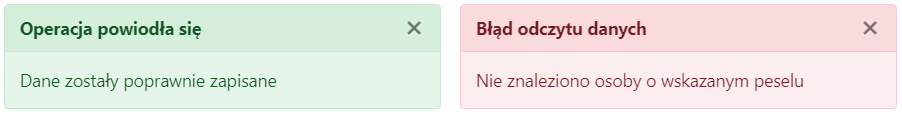
\includegraphics[width=130mm]{figures/komunikaty.PNG}
\caption{Przykładowe komunikaty prezentowane użytkownikowi}
\label{fig:komunikaty}
\end{figure}

Rysunek \ref{fig:examleForm} przedstawia ekran z przykładowo uzupełnionym formularzem. Uzupełnione zostały wszystkie \textit{Dane osobowe} pacjenta, a dane kontaktowe zostały pominięte. Została sprawdzona poprawność pól wymaganych - \textit{Pierwsze imię}, \textit{Nazwisko} oraz \textit{Pesel} zaznaczone są kolorem zielonym, co oznacza, że mają prawidłowy format. \textit{Data urodzenia} została automatycznie uzupełniona na podstawie podanego peselu.


\subsubsection{Diagram zębowy}

Drugi w kolejności widok, znajdujący się w zakładce \textit{Diagram zębowy}, prezentuje dwa diagramy. Domyślnie wyświetlane są zęby stałe, ale dostępny jest także diagram zębów mlecznych. By ułatwić korzystanie z aplikacji, w górnej części ekranu znajdują się podstawowe dane pacjenta wprowadzone w formularzu. Nad diagramem, po prawej stronie, umieszczone są przyciski umożliwiające przełączanie pomiędzy różnymi wersjami zapisanych danych. Podczas kolejnych wizyt stomatolog lub jego asystent zapisuje dane jako kolejne ich wersje, do których później ma dostęp dzięki wskazanym przyciskom. Wersje oznaczane są datą i godziną. Rysunek \ref{fig:diagram} prezentuje dane zapisane 17 stycznia 2021 roku o godzinie 17:30.

\begin{figure}[ht!]
\centering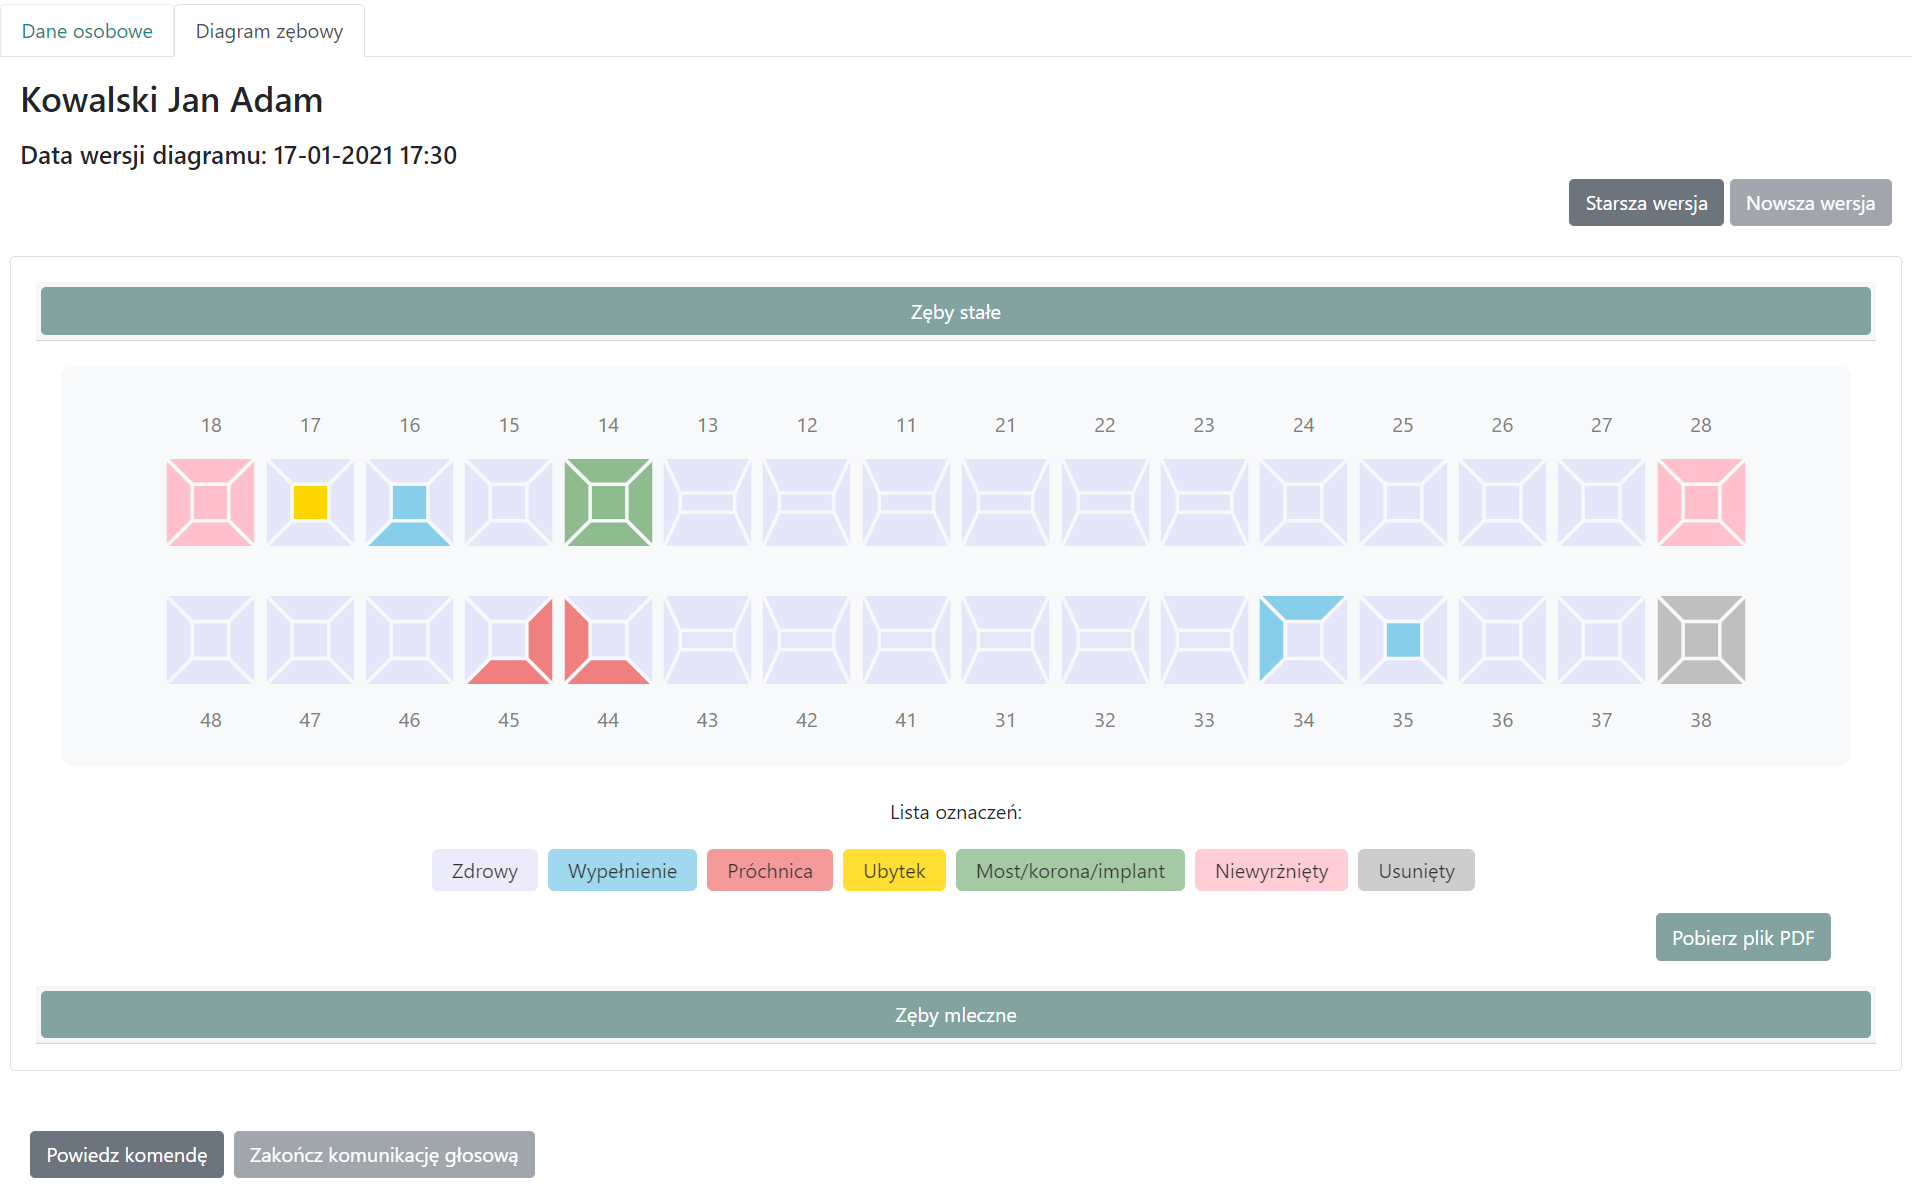
\includegraphics[width=\textwidth]{figures/diagram.PNG}
\caption{Ekran prezentujący diagram zębowy pacjenta}
\label{fig:diagram}
\end{figure}

Głównym elementem drugiego ekranu jest diagram zębowy. Składa się on z trzydziestu dwóch zębów w przypadku diagramu zębów stałych oraz dwudziestu zębów tworzących diagram zębów mlecznych. Użytkownik ma możliwość wybrania zęba, który powiększa się po najechaniu na jego powierzchnię, oraz jednej z pięciu jego części. Kliknięcie wybranego elementu otwiera listę możliwych do wyboru chorób. Po wybraniu jednej z nich część zęba oznaczana jest odpowiednim kolorem. By zwiększyć czytelność diagramu, pod zębami znajduje się lista objaśniająca poszczególne barwy.

Oprócz możliwości wprowadzania danych przy pomocy myszki użytkownik może skorzystać z dostępnego w aplikacji interfejsu głosowego. By aktywować działanie interfejsu trzeba użyć przycisku \textit{Powiedz komendę}, a zakończyć nasłuchiwanie można przyciskiem \textit{Zakończ komunikację głosową} lub wypowiadając komendę \textit{STOP}. Zrozumiane przez system komendy zostają w czasie rzeczywistym nanoszone na diagram. Dodatkowo, w prawym górnym rogu ekranu, w formie komunikatów, wyświetlane są wprowadzane właśnie zmiany. Działanie interfejsu głosowego nie wyklucza możliwości nanoszenia zmian przy użyciu myszki. Obu sposobów można z powodzeniem używać w tym samym czasie. Rysunek \ref{fig:zmiany} pokazuje zmiany wprowadzone na diagramie oraz wyświetlane komunikaty po wypowiedzeniu dwóch komend głosowych - \textit{osiemnaście policzkowa ubytek} oraz \textit{dwadzieścia osiem cały implant}.

\begin{figure}[ht!]
\centering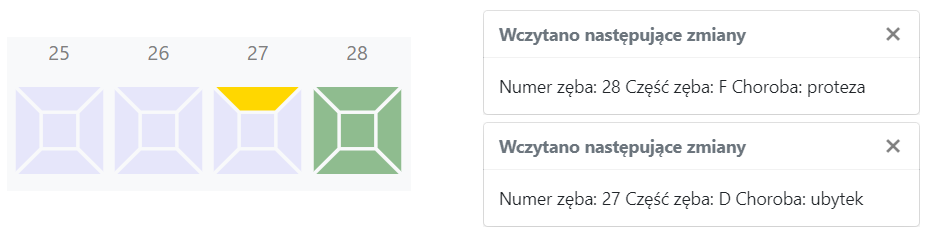
\includegraphics[width=130mm]{figures/zmiany.PNG}
\caption{Przykładowe zmiany wprowadzone przez użytkownika przy pomocy interfejsu głosowego}
\label{fig:zmiany}
\end{figure}

Dodatkowo, by umożliwić przekazywanie danych między pracownikami służby zdrowia, ale także dać możliwość udostępniania danych pacjentom, na ekranie dostępny jest przycisk \textit{Pobierz plik PDF}. Pozwala on na zapis danych do pliku, który można następnie łatwo udostępnić (Rysunek \ref{fig:pdf}).

\begin{figure}[ht!]
\centering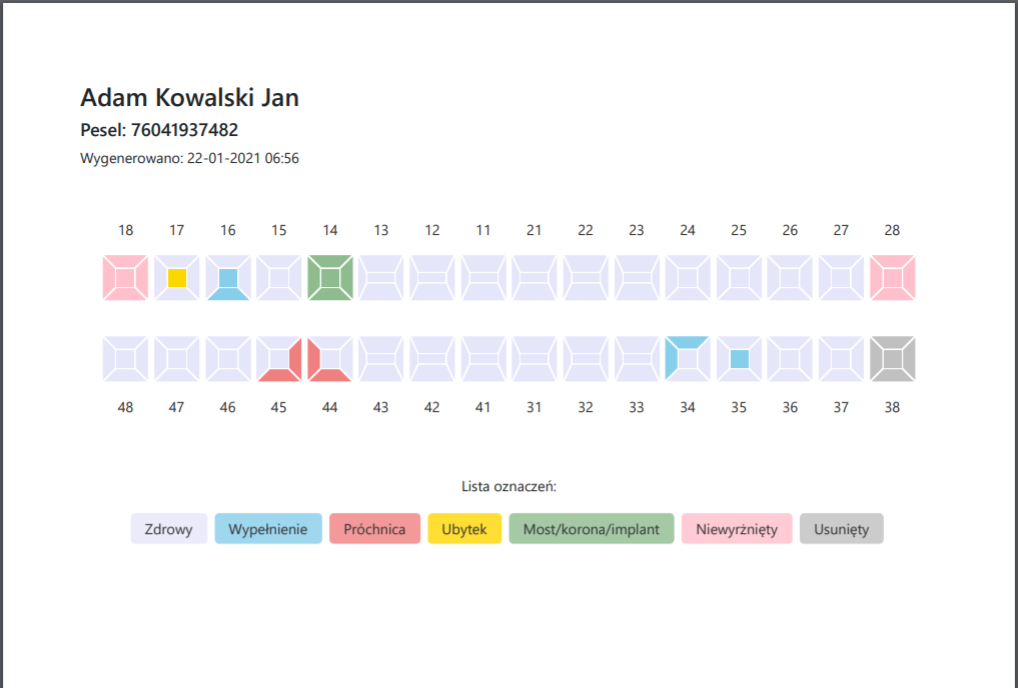
\includegraphics[width=130mm]{figures/pdf.png}
\caption{Fragment wygenerowanego automatycznie pliku PDF.}
\label{fig:pdf}
\end{figure}


\section{Analiza odchylenia toru odwodzenia żuchwy}
\subsection{Wymagania}
W tym module również założono minimalne wymagania produktowe - MVP:
\begin{itemize}
    \item Automatyczne wykrycie górnych i~dolnych zębów
    \item Obliczenie maksymalnego wychylenia żuchwy od stanu początkowego (zaciśniętych zębów) podczas odwodzenia i przywodzenia żuchwy w kątach i milimetrach
    \item Eksportowanie danych do pliku w~formacie pdf
\end{itemize} 
\subsection{Design}
\subsection{Proces instalacji i~uruchomienia}
   \begin{itemize}
    \item zmienić readme w~coś sensownego do czytania :P
    
\end{itemize} 
\subsection{Trudności}
\subsection{Testy}
\subsection{Przykłady użycia}